% !TEX root = ..\Main.tex
\chapter{Formal Definitions}
\label{chapterlabel:Definitions}

\section{Notation and Computational Model}

This thesis is concerned with algorithms modelled as probabilistic polynomial-time Turing machines, and interactive probabilistic polynomial-time Turing machines. We use the abbreviations PPT and DPT for algorithms running in probabilistic polynomial time and deterministic polynomial time respectively, where the running time is polynomial in the size of the algorithm inputs. Unless otherwise stated, the sizes of inputs and outputs to the machines will be bounded above by a polynomial in a security parameter $\sep$, usually provided to the algorithms in unary form as $1^\sep$.

For functions $f,g: \N \rightarrow [0,1] $, we write $f(\sep)\approx g(\sep) $ if 
$|f(\sep) - g(\sep)|= \frac{1}{\sep^{\omega(1)}}$. We say a function $f$ is \emph{overwhelming} if 
$f(\sep) \approx 1$ and $f$ is \emph{negligible} if $f(\sep) \approx 0$.

Write $y=A(x;r)$ when the algorithm $A$ outputs $y$ on input $x$ with randomness $r$. We write $y \gets A(x)$ to mean selecting $r$ at random and setting $y=A(x;r)$. We write $y \gets S$ for sampling $y$ uniformly at random from a set $S$. We define $[n]$ to be the set of integers $1,\ldots,n$.

We use $\F$ to denote a finite field. We use bold letters such as $\vec{v}$ for row vectors. For $\vec{v}\in \F^n$ and a set $J=\{j_1,\dots, j_k\}\subset [n]$ with $j_1<\dots<j_k$ we define the vector $\vec{v}|_J$ to be $(\vec{v}_{j_1},\dots, \vec{v}_{j_k})$. Similarly, for a matrix $V\in \F^{m\times n}$ we let $V|_{J}\in \F^{m\times k}$ be the submatrix of $V$ restricted to the columns indicated in $J$.

Let $z_1,\ldots,z_m$ be distinct points in a finite field $\F$. and let $l_1(X),\ldots,l_m(X)$ be their associated Lagrange polynomials. Explicitly, $$l_i(X) = \prod_{j \neq i} \frac{X-z_j}{z_i - z_j}$$ Note that $l_i(z_j)=\delta_{i,j}$, so it is easy to see how to combine the Lagrange polynomials to produce a polynomial which interpolates a given function at $z_1, \ldots, z_m$. Let $l_0(X) = \prod_{i=1}^m (X-z_i)$. 

\section{Zero-Knowledge Proofs}
\label{shvzkdef}

A \emph{proof system} is defined by a triple of stateful PPT algorithms $(\mathcal{K},\mathcal{P},\mathcal{V})$, which we call the common-reference-string \emph{generator}, the \emph{prover} and \emph{verifier}, respectively.

The setup generator $\mathcal{K}$ creates public parameters $\crs$ which provide the necessary setup information for \prover and \verifier to run the protocol. On input $1^\lambda$, the generator $\crsgen$ produces a common reference string $\crs$. We think of $\crs$ as being honestly generated and use the public parameter model purely for simplicity and efficiency in our proofs. However, in the proofs we construct, $\crs$ consists of parts that are either publicly verifiable or could be generated by the verifier, so we do not rely on the public parameter model for security in any way.

The prover and verifier communicate with each other through a \emph{communication channel} $\overset{\textnormal{chan}}{\longleftrightarrow}$. When $\mathcal{P}$ and $\mathcal{V}$ interact on inputs $s$ and $t$ through a communication channel $\overset{\textnormal{chan}}{\longleftrightarrow}$ we let $\viewV \leftarrow \langle \mathcal{P}(s) \overset{\textnormal{chan}}{\longleftrightarrow} \mathcal{V}(t)\rangle$ be the view of the verifier in the execution, which is made up of all of the verifier's inputs, including random coins, and let $\viewp \leftarrow  \langle \mathcal{P}(s) \overset{\textnormal{chan}}{\longleftrightarrow} \mathcal{V}(t)\rangle$ denote the transcript of the communication between prover and channel. This overloads the notation $\leftarrow  \langle \mathcal{P}(s) \overset{\textnormal{chan}}{\longleftrightarrow} \mathcal{V}(t)\rangle$ but it will always be clear from the variable name if we get the verifier's view or the prover's transcript. At the end of the interaction the verifier accepts or rejects. We write $\langle \mathcal{P}(s)\overset{\textnormal{chan}}{\longleftrightarrow} \mathcal{V}(t)\rangle =b$ depending on whether the verifier rejects ($b=0$) or accepts ($b=1$).

In the \emph{standard channel} $\std$, all messages are forwarded between prover and verifier. 
We also consider an \emph{ideal linear commitment}  channel, \ILC, described in Figure~\ref{ILCSyntaxFigure11}. 
When using the \ILC\ channel, the prover can submit a \ILCcommit\ command to commit to 
vectors of field elements of some fixed length $\sizevect$, specified in $\crs_{\ILC}$. The vectors remain secretly stored in the channel, and will not be forwarded to the verifier. Instead, the verifier only learns how many vectors the prover has committed to, and their lengths. The verifier can submit a \ILCsend\ command to the \ILC\ to send field elements to the prover. In addition, the verifier can also submit \ILCopen\ queries to the \ILC\ for obtaining the opening of any linear combinations of the vectors \emph{of the same length} sent by the prover. We stress that the verifier can request several linear combinations within a single \ILCopen\ query, as depicted in Figure~\ref{ILCSyntaxFigure11}.

In addition to the \ILC\ commands used in the original model \cite{BootleCGGHJ17}, we introduce the new command \ILCcheck. Inside the \ILC \ model, this command behaves in an identical way to the \ILCsend\ command. However, the two commands will be treated slightly differently when \ILC\ protocols are compiled into real protocols. The reason for making the distinction is that in some of our protocols, the verifier needs to check whether a large vector, that they have computed themselves, is the correct linear combination of vectors committed by the prover. This could be solved by having the verifier make an \ILCsend\ query for the correct linear combination and checking whether the result is equal to the large vector, which incurs a communication cost for the large vector in the \ILC\ protocol. However, in a real protocol, where the verifier's queries will actually be computed and sent by the prover, the verifier can re-commit to the vector that they have computed, and check against the prover's commitments. In other words, since the verifier has already computed the vector for themself, there is no need for them to receive it again. Therefore, the \ILCcheck\ command is used to distinguish this case, which should not be counted as part of the communication costs of a proof. This issue will be discussed further in later chapters.

\begin{figure}[htb]
\resizebox{\textwidth}{!}{\begin{tabular}{lll}
$\Po_{\ILC~}$ &\multirow{4}{*}{ \resizebox{0.8\linewidth}{!}{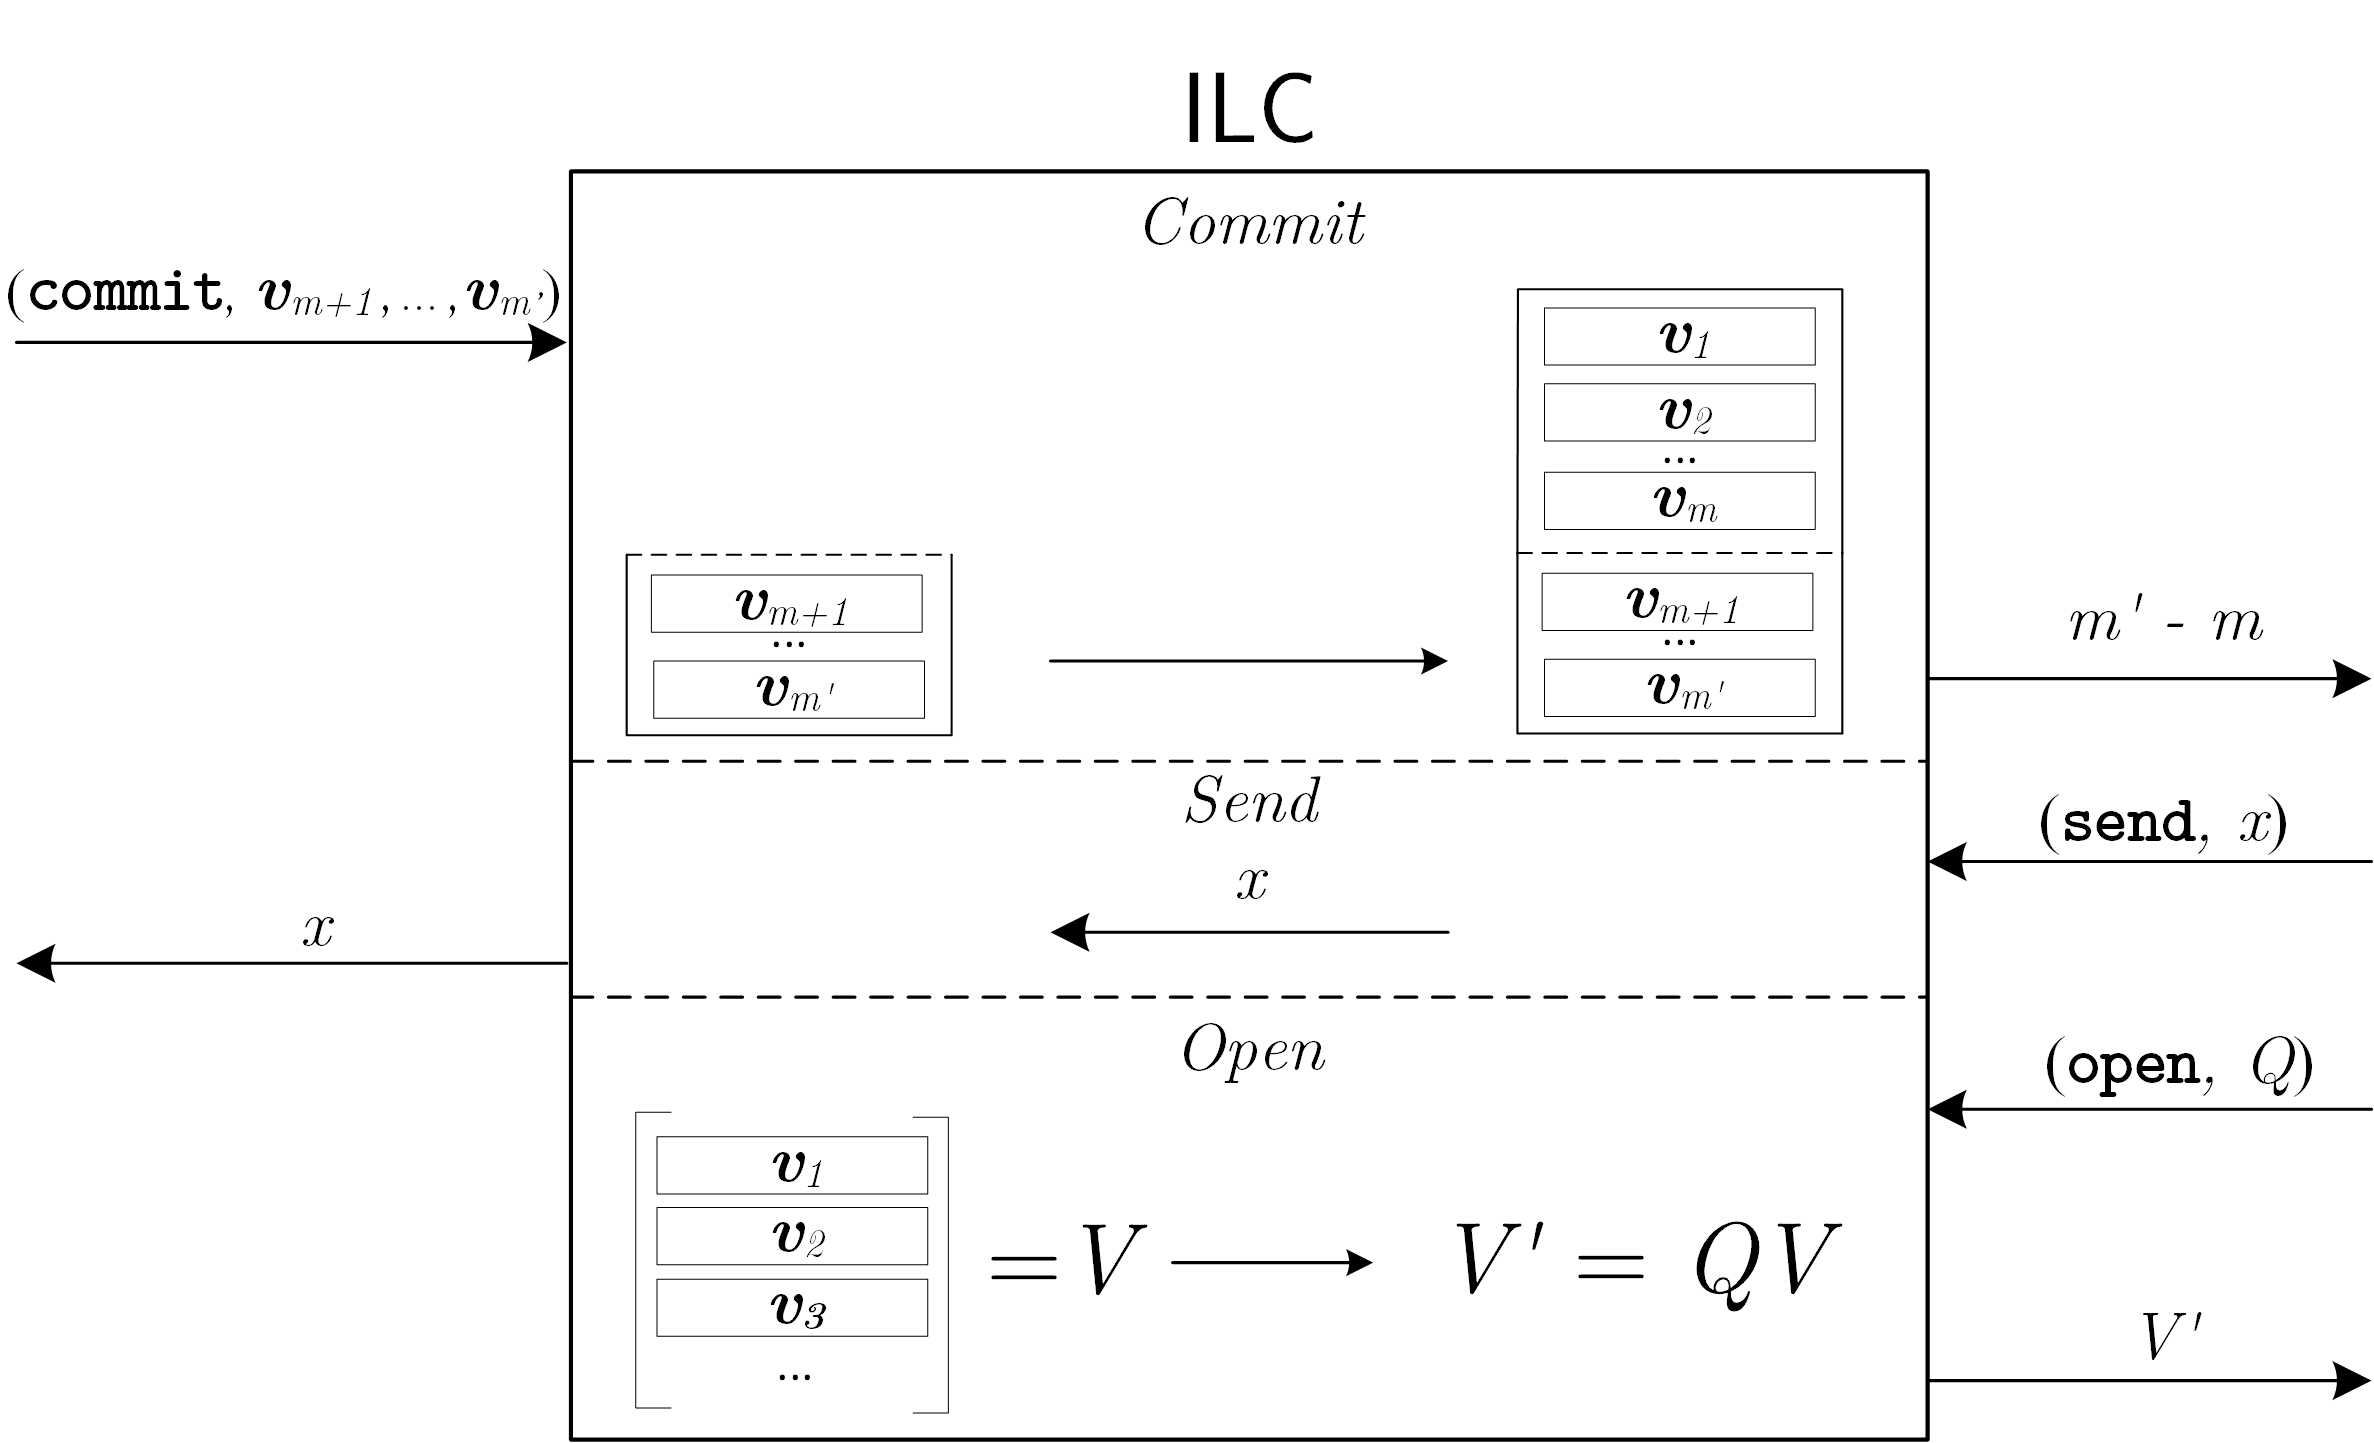
\includegraphics{ILC2-shrink.png}} }&$\V_{\ILC~}$\\
&& \\&&\\&&\\&&\\&&\\&&\\&&\\&&\\&&\\&&\\&&\\
&&\\&&\\
\end{tabular}}\caption{Description of the $\ILC~$ channel.}\label{ILCSyntaxFigure11}
\end{figure}

In a proof system over the \ILC\ channel, sequences of \ILCcommit, \ILCsend\ and \ILCopen\ and \ILCcheck\ queries could alternate in an arbitrary order. We call a proof system over the \ILC\ channel \emph{non-adaptive} if the verifier makes one \emph{open} query and then immediately makes one \emph{check} query to the \ILC\ channel, before terminating his interaction with the channel, and these are the only \emph{open} and \emph{check} queries that the verifier makes. Otherwise we call it \emph{adaptive}. Although adaptive proof systems are allowed by the model, in this paper we will only consider non-adaptive \ILC\ proof systems to simplify the exposition. In non-adaptive \ILC\ proof systems with vectors of length $\sizevect$, the verifier will produce two query matrices, $Q$ for the \ILCopen\ query and $Q$ for the \ILCcheck\ query. 

In fact, in our protocols, we will allow the prover to commit to vectors of \emph{several different fixed lengths} $\sizevect_1,\ldots,\sizevect_r$, which will be specified at the beginning of the protocol. This is easily formalised by defining a new communication channel, giving the prover and verifier access to $r$ copies of different \ILC\ channels of lengths $\sizevect_1,\ldots,\sizevect_r$. For the new channel, the \ILCcommit\ command on vectors $\vec{v}_1,\ldots,\vec{v}_m$ separates the vectors into sets of vectors of lengths $\sizevect_1,\ldots,\sizevect_r$, and commits to the set of vectors of length $\sizevect_i$ using the $i$th \ILC\ channel on vectors of length $\sizevect_i$. The \ILCsend\ command for the new channel simply takes the verifier's message and sends it to each of the $r$ \ILC\ channels using their own \ILCsend\ command. For the \ILCopen\ and \ILCcheck\ commands for the new channel, the verifier's queries take the form $Q = (Q_1,\ldots,Q_r)$, where each $Q_i$ is a query matrix for the $i$th \ILC\ channel. The new channel returns the responses of all of the \ILC\ queries to the verifier. Such a channel will be referred to as an \ILC\ channel for vectors of several fixed lengths, and will be specified simply by including multiple vector lengths in $\crs_{\ILC~}$ rather than just one.

Alternatively, we can easily incorporate vectors of different lengths into the model by padding all vectors with zeroes until they are the same length as the longest vector. This will have no impact on the asymptotic efficiency of our protocols. Some of our \ILC\ protocols require single values to be committed as well as vectors. 

We remind the reader that \ILC\ proof systems are different from linear interactive proofs considered in \cite{BitanskyCIPO13}. In linear interactive proofs both the prover and verifier send vectors of field elements, but the prover can only send linear (or affine) transformations of the verifier's previously sent vectors. However, for our constructions it is important that the prover can compute on field elements received by the verifier and for instance evaluate polynomials.

We say a proof system is \emph{public coin} if the verifier's messages to the communication channel are chosen uniformly at random and independently of the actions of the prover, i.e., the verifier's messages to the prover correspond to the verifier's randomness $\rho$.

We will model our zero-knowledge proofs using ternary relations $\R$ consisting of tuples $(\crs, \stm,\wit)$. The first item in the tuple is the \emph{common reference string} $\crs$ containing the setup information required for the protocol. Typically, $\crs$ will specify the security parameter $\sep$, perhaps implicitly through its length, and may also contain other parameters used for specifying the specific relation, e.g. a description of a field. Often, $\crs$ will also contain parameters that do not influence membership of $\R$ but may aid the prover and verifier, for instance, a description of an encoding function that they will use. The second item in the tuple, $\stm$ is the \emph{instance} and represents what the prover wants to prove. The final item, $\wit$, is the prover's secret \emph{witness} that $(\crs,\stm)\in\LL_\R$ where the language $\LL_\R \subset \{0,1\}^*$ as follows.
\[ \LL_\R=\{(\crs,\stm)|\exists \wit: (\crs,\stm,\wit)\in \R\} \]
Intuitively speaking, this is the collection of statements which are `true', and for which the verifier should output one after running the protocol with an honest prover. The languages $\LL_\R$ are decidable in polynomial time.

The protocol $(\KK,\mathcal{P},\mathcal{V})$ is called a \emph{proof of knowledge} over communication channel $\overset{\textnormal{chan}}{\longleftrightarrow}$ for relation $\R$ if it has perfect completeness and computational knowledge soundness as defined below.

\begin{definition}[Perfect Completeness]
The proof is \emph{perfectly complete} if for all PPT adversaries $\mathcal{A}$
$$\Pr \left[ \begin{array}{c} \crs\gets \KK(1^\sep); (u,w) \leftarrow \mathcal{A}(\crs): \\
(\crs,u,w)\notin \R ~\vee~ \langle \mathcal{P}(\crs,u,w)\overset{\textnormal{chan}}{\longleftrightarrow}\mathcal{V}(\crs,u)\rangle=1 \end{array}\right] =1.$$
\end{definition}

\begin{definition}[Knowledge soundness]
A public-coin proof system has \emph{computational (strong black-box) knowledge soundness} if for all DPT $\Po^*$ there exists an expected PPT extractor $\E$ such that for all PPT adversaries $\A$
$$\Pr\left[\begin{array}{c} \crs\gets \KK(1^\sep);(\stm,s) \gets \mathcal{A}(\crs); \wit\gets \E^{\langle \Po^*(s)\overset{\textnormal{chan}}{\longleftrightarrow}\V(\crs,\stm)\rangle}(\crs,\stm):\\ b=1 ~\wedge~ (\crs,\stm,\wit)\notin \R \end{array}\right]\approx 0.$$ 
Here the oracle $\langle \Po^*(s)\overset{\textnormal{chan}}{\longleftrightarrow}\V(\crs,\stm)\rangle$ runs a full protocol execution and if the proof is successful it returns a transcript of the prover's communication with the channel. The extractor $\E$ can ask the oracle to rewind the proof to any point in a previous transcript and execute the proof again from this point on with fresh public-coin challenges from the verifier. We define $b\in \{0,1\}$ to be the verifier's output in the first oracle execution, i.e., whether it accepts or not, and we think of $s$ as the state of the prover. The definition can then be paraphrased as saying that if the prover in state $s$ makes a convincing proof, then we can extract a witness.

If the definition holds also for unbounded $\mathcal{P}^*$ and $\A$ we say the proof has {\em statistical knowledge soundness}. 

If the definition of knowledge soundness holds for a non-rewinding extractor, i.e., a single transcript of the prover's communication with the communication channel suffices, we say the proof system has knowledge soundness with {\em straight-line extraction}. 
\end{definition}
\noindent
This definition gives a security guarantee against computationally bounded adversaries. Zero-knowledge protocols satisfying this definition are properly called zero-knowledge arguments of knowledge to distinguish them from zero-knowledge proofs of knowledge, for which knowledge soundness is guaranteed even against unbounded adversaries. However, the term `proofs' is often used in both cases.

Another way to define a proof of knowledge follows Groth and Ishai~\cite{GrI08} who borrowed the term witness-extended emulation from Lindell~\cite{Lin03}. Informally, their definition says that given an adversary that produces an acceptable argument with some probability, there exists an emulator that produces a similar argument with the same probability together with a witness $w$. Note that the emulator is allowed to rewind the prover and verifier's interaction to any previous move.

\begin{definition}[Witness-extended emulation]
$(\mathcal{P},\mathcal{V})$ has {\em statistical witness-extended emulation} if for all deterministic polynomial time $\mathcal{P}^*$ there exists an expected polynomial time emulator $\mathcal{E}$ such that for all interactive adversaries $\mathcal{A}$
\begin{align*}
& \Pr \Big{[}(u,s) \leftarrow\mathcal{A}(1^\sep); tr \leftarrow \langle \mathcal{P}^*(u,s), \mathcal{V}(u)\rangle: \mathcal{A}(tr)=1 \Big{]}\\
\approx \ & \Pr \left[ \begin{array}{l} (u,s) \leftarrow \mathcal{A}(1^\sep); (tr,w) \leftarrow \mathcal{E}^{ \langle \mathcal{P}^*(u,s), \mathcal{V}(u) \rangle } (u): \\ \mathcal{A}(tr)=1 \text{\emph{ and if }} tr \text{\emph{ is accepting then }} (u,w) \in R \end{array} \right]
\end{align*}
where the oracle called by $\mathcal{E}^{\langle \mathcal{P}^*(u,s), \mathcal{V}(u)\rangle}$ permits rewinding to a specific point and resuming with fresh randomness for the verifier from this point onwards.
\end{definition}
\noindent
Note that in this definition, the role of the adversary $\mathcal{A}$ is as a distinguisher, while it is the job of $\mathcal{P}^*$ to produce proofs. That is why the two are decoupled from one another.

We can interpret $s$ as the state of $\mathcal{P}^*$, including the randomness. So, whenever $\mathcal{P}^*$ is able to make a convincing argument when in state $s$,  $\mathcal{E}$ can extract a witness. Witness Extended Emulation implies Knowledge Soundness \cite{dissertation}.

We will construct public-coin proofs that have special honest-verifier zero-knowledge. This means that if the verifier's challenges are known, or even adversarially chosen, then it is possible to simulate the verifier's view without the witness.  In other words, the simulator works for verifiers who may use adversarial coins in choosing their challenges but they follow the specification of the protocol as an honest verifier would. 
\begin{definition}[Special Honest-Verifier Zero-Knowledge]
The proof of knowledge is \emph{computationally special honest-verifier zero-knowledge (SHVZK)} if there exists a PPT simulator $\mathcal{S}$ such that for all stateful interactive PPT adversaries $\mathcal{A}$ that output $(u,w)$ such that $(\crs,u,w)\in R$ and randomness $\rho$ for the verifier
\begin{eqnarray*}
&&\Pr \left[ \begin{array}{c}\crs\gets \KK(1^\sep);(u, w, \rho) \leftarrow\mathcal{A}(\crs); \\
\viewV\leftarrow \langle \mathcal{P}(\crs,u,w)\overset{\textnormal{chan}}{\longleftrightarrow} \V(\crs,u;\rho)\rangle: \A(\viewV)=1\end{array} \right]\\
&\approx &\Pr \left[ \crs\gets \KK(1^\sep);(u, w, \rho) \leftarrow\mathcal{A}(\crs); \viewV\leftarrow \mathcal{S}(\crs,u,\rho): \mathcal{A}(\viewV)=1\right].
\end{eqnarray*}

We say the proof is \emph{statistically SHVZK} if the definition holds also against unbounded adversaries, and we say the proof is \emph{perfect SHVZK} if the probabilities are exactly equal.
\end{definition}


\heading{\bf From Honest-Verifier to General Zero-Knowledge}
Honest-verifier zero-knowledge only guarantees that the simulator works for verifiers following the proof system specifications. It might be desirable to consider general zero-knowledge where the simulator works for arbitrary malicious verifiers that may deviate from the specification of the proof. However, honest-verifier zero-knowledge is a first natural stepping stone towards efficient zero-knowledge proofs. %and it depends on the situation how you would want to proceed to get full zero-knowledge. 
 We recall that our proofs are public coin, which means that the verifier's messages are chosen uniformly at random and independently from the messages received from the verifier. Below we recall few options to obtain general zero-knowledge proofs from a public-coin SHVZK proof. All these transformations are very efficient in terms of computation and communication such that the efficiency properties of our special honest-verifier zero-knowledge protocols are preserved. 

In the Fiat-Shamir transform \cite{FiatShamir} the verifier's challenges are computed using a cryptographic hash function applied to the transcript up to the challenge. The Fiat-Shamir transform is more generally used to turn a public-coin proof into a non-interactive one. Since interaction with the verifier is no longer needed, general zero-knowledge is immediately achieved. The drawback of the Fiat-Shamir transform is that security is usually proved in the random oracle model \cite{bellarerogaway} where the hash function is modelled as an ideal random function.% truly random message digests.

Other transformations such as \cite{Damgard2000,MP03,GoldreichSV98} have already been discussed.
%
%Assuming a common reference string and relying on trapdoor commitments, Damg{\aa}rd \cite{Damgard2000} gave a transformation yielding concurrently secure protocols for $\Sigma$-Protocols. The transformation can be optimized~\cite{dissertation} using the idea that for each public-coin challenge $x$, the prover first commits to a value $x'$, then the verifier sends a value $x''$, after which the prover opens the commitment and uses the challenge $x=x'+x''$. The coin-flipping can be interleaved with the rest of the proof, which means the transformation preserves the number of rounds and only incurs a very small efficiency cost to do the coin-flipping for the challenges. 
%
%If one does not wish to rely on a common reference string for security, one can use a private-coin transformation where the verifier
%does not reveal the random coins used to generate the challenges sent to the prover (hence the final protocol is no longer public coin).
%One example is the Micciancio and Petrank \cite{MP03} transformation (yielding concurrently secure protocols) while incurring a small overhead of $\omega(\log{\lambda})$ with respect to the number of rounds as well as the computational and communication cost in each round. % where $\lambda$ is the security parameter and $\omega(\log{\lambda})$ is independent of the complexity of the original protocol. 
%The transformation preserves the soundness and completeness errors of the original protocol; however, it does not preserve statistical zero-knowledge as the obtained protocol only has computational zero-knowledge. 
%
%There are other public-coin transformations to general zero-knowledge e.g.~Goldreich et al.~\cite{GoldreichSV98}. The transformation relies on a random-selection protocol between the prover and verifier to specify a set of messages and restricting the verifier to choose challenges from this set. This means to get negligible soundness error these transformations require $\omega(1)$ sequential repetitions so the round complexity goes up. 
%
\section{Arithmetic Circuits}\label{sec:AC}

Arithmetic circuits are a model for algebraic computation over fields. An arithmetic circuit consists of addition and multiplication gates. Our satisfiability arguments consider arithmetic circuits described as a list of multiplication gates together with a set of linear consistency equations relating the inputs and outputs of the gates. 
%
In this section, we show how to reduce an arbitrary arithmetic circuit to this format.

\begin{definition} An arithmetic circuit over a field $\F$ and variables $(A_1,\ldots,A_m)$ is a directed acyclic graph whose vertices are called gates. Gates of in-degree 0 are inputs to the circuit and labelled with some $A_i$ or a constant field element. All other gates are labelled $+$ or $\times$.
\end{definition}

Given field elements $a_i \in \F$, an arithmetic circuit is evaluated in several steps. First, label the inputs with the $a_i$. Then, take gates whose inputs are all labelled with field elements, apply the operation on the gate to the inputs and write the answer on the output wire. and repeating this process until all gates have been labelled with output field elements.

We may consider fan-in 2 circuits, in which case all of the $+$ and $\times$ gates have in-degree 2, or arbitrary fan-in circuits. We consider circuits with arbitrary fan-out, in which case all of the $+$ and $\times$ gates have unbounded out-degree.

Arithmetic circuits can be measured in various ways. The size of an arithmetic circuit is the number of gates in the circuit. This can be further split into the number of addition gates and the number of multiplication gates. The depth of a circuit is the length of the longest path beginning from any circuit input. It is easy to see that arithmetic circuits compute polynomial functions of their inputs, and the degree of the arithmetic circuit is the total degree of the polynomial that it computes.

Arithmetic circuits can be described alternatively as a list of multiplication gates with a collection of linear consistency equations relating the inputs and outputs of the gates. Our zero-knowledge protocols for circuit satisfiability use circuits in this form. Any circuit described as an acyclic graph can be efficiently converted into the alternative description.

At a high level, we transform an arithmetic circuit into two kinds of equations. 
Multiplication gates are directly represented as equations of the form $a\cdot b=c$, where $a,b,c$ represent the left, right and output wires. We will arrange these values in matrix form producing a Hadamard matrix product. This process will lead to duplicate values, when a wire is the output of one multiplication gate and the input of another, or when it is used as input multiple times. We keep track of this by using a series of linear constraints. For example, suppose we have two multiplication gates with wire values $a_1,b_1,c_1$ and $a_2,b_2,c_2$. If the output of the first multiplication gate is the right input of the second, we would write $c_1 - b_2 = 0$.

We also add linear constraints representing the addition and multiplication by constant gates of the circuit. We then rewrite those equations so that the only wires that are referenced in the equations are those linked to (non-constant) multiplication gates. %This is always possible if we allow for some preprocessing of the initial circuit. 
We now describe this process.

\subsection{Reduction of Circuit Satisfiability Problem to a Hadamard Matrix Product and Linear Constraints.}
We consider an arithmetic circuit containing $N=mn$ multiplication gates over a field $\F$. Without loss of generality, we assume that the circuit has been pre-processed as in the next section, so that the input and the output wires feed into and go out from multiplication gates only.
We number the multiplication gates from 1 to $N$ and we arrange the inputs and outputs of these gates into three $m\times n$ matrices $A,B$ and $C$ such that the $(i,j)$ entries of the matrices correspond to the left input, right input and output of the same multiplication gate.

As shown in \cite{BootleCCGP16}, an arithmetic circuit can be described as a system of equations in the entries of the above matrices. The multiplication gates define a set of $N$ equations 
\begin{equation}\label{eq1:product}
A \circ B = C
\end{equation}
where $\circ$ is the Hadamard (entry-wise) product. 
%
The circuit description also contains constraints on the wires between multiplication gates. %The output of one multiplication gate might feed into a combination of addition gates and multiplication by constant gates yielding one or more inputs to other multiplication gates. 
Denoting the rows of the matrices $A,B,C$ as
\begin{align*}\vec{a}_ {i}=(a_{i,1},\ldots,a_{i,n})&& \vec{b}_ {i}=(b_{i,1},\ldots,b_{i,n})&&\vec{c}_ {i}=(c_{i,1},\ldots,c_{i,n})&& \text{for }  i \in \{1,\ldots,m\}\end{align*}
these constraints can be expressed as $Q<2N$ linear equations of inputs and outputs of multiplication gates of the form
\begin{equation}\label{eq1:consistency}
\sum_{i=1}^m \vec{a}_{i} \cdot \vec{w}_{q,{a,i}}+\sum_{i=1}^m \vec{b}_{i} \cdot \vec{w}_{q,{b,i}}+\sum_{i=1}^m \vec{c}_{i} \cdot  \vec{w}_{q,{c,i}}=K_{q} \quad \text{ for } q \in\{1,\ldots,Q\}
\end{equation}
for constant vectors $\vec{w}_{q,{a,i}},\vec{w}_{q,{b,i}},\vec{w}_{q,{c,i}}$ and scalars $K_{q}$.

For example, suppose that the circuit contains a single addition gate, with $a_{1,1}$ and $a_{1,2}$ as inputs, and $b_{1,1}$ as output. In this case, $Q=1$ and we would set $\vec{w}_{1,a,1} = (1,1,0,\ldots,0)$, $\vec{w}_{1,b,1} = (-1,0,\ldots,0)$, and all other $\vec{w}$ vectors would be set to $\vec{0}$. Then~\eqref{eq1:consistency} would simply read
$$ a_{1,1} + a_{1,2} - b_{1,1} = 0$$
to capture the constraint imposed by the addition gate.

In total, to capture all multiplications and linear constraints, we have $N+Q$ equations that the wires must satisfy in order for the circuit to be satisfiable. %We can combine the equations into a polynomial of degree $N+Q$ in an indeterminate $Y$ such that the circuit is satisfiable if and only if the polynomial is identically 0.

\subsection{Preprocessing Arithmetic Circuits for Arguments}\label{sec:preprocAC}

We show how to remove addition and multiplication-by-constant gates  from an arithmetic circuit $A$, and replace them with bilinear consistency equations on the inputs and outputs of the remaining gates, such that satisfiability of the equations is equivalent to satisfiability in the original circuit.

 Let $B$ be the sub-circuit of $A$ containing all wires and gates before a multiplication gate, with $m$ input wires and $n$ output wires. Label the $m$ inputs of $B$ with the unit vectors $\vec{e}_i=(0,\ldots,1,\ldots,0)$ of length $m$. For every addition gate with inputs labelled as $\vec{x},\vec{y}$, label the output wire as $\vec{x}+\vec{y}$. For every multiplication-by-constant gate with inputs $\vec{x}$ and constant $c$ label the output with $c\vec{x}$. By proceeding inductively, the $n$ outputs of $B$ are now labelled with vectors of length $m$ representing them as linear combinations of the inputs.

This requires at most $m\left| B \right|$ arithmetic operations. Note however that all outputs of $B$ are linear combinations of the inputs, and that $B$ can be written with $n(2m-1)$ fan-in 2 gates in such a way that the consistency equations can be trivially read off from the circuit description. More specifically, a linear combination $\sum_{i=1}^m a_i x_i$ can be produced using $m$ multiplication-by-constant gates and $m-1$ addition gates to add the answers together.

We can now remove the gates of $B$ from $A$. We also remove any multiplication gates whose inputs are the inputs of the new circuit. Now we simply repeat the process of finding consistency equations until we have considered the whole of~$A$. In Figure~\ref{fig:digraph} there is an example of a circuit together and the corresponding consistency equations.



The first (input) and final (output) sub-circuits require additional processing. We show how to do this for the output sub-circuit. The input sub-circuit is very similarly handled.

Let $B$ be the output sub-circuit. Write $(a_1,\ldots,a_m)=\vec{a}$ for the input wires of $B$ and $(b_1,\ldots,b_n)=\vec{b}$ for the output wires. Without loss of generality, we may ignore variable output wires. By construction of $B$, each output $b_i$ is of the form $\sum_{i=1}^n q_{ij}a_j+p_i$, with consistency equations obtained as above. We write this in terms of an $m\times n$ matrix $\mathsf{Q}$ and a column vector $\vec{p}$ of size $m$, namely
$$\vec{b} = \mathsf{Q} \vec{a}+ \vec{p}.$$
%
Let $r$ be the rank of $\mathsf{Q}$. We convert $\mathsf{Q}$ into reduced row echelon form $\mathsf{R}$, writing
$$\vec{b''}=\mathsf{R}\vec{a}.$$

By the properties of reduced row echelon form, after relabelling the $a_i$ and permuting the columns of $\mathsf{R}$ to match, we have that $b''_i=a_i + \sum_{j=l+1}^m r_{ij} a_j$ for $1\leq i\leq l$. Therefore, we may consider $a_{l+1},\ldots,a_m$ as free wires and express other $a_i$ as linear functions of these wires plus constants.

Note that if $b''_i\neq 0$ for some $i>l$, the circuit can never be satisfied anyway. However, assuming that our statement is a satisfiable circuit, with a witness consisting of satisfying wire values, this never occurs. Then the original circuit is satisfied if and only if the $a_i$ values satisfy the consistency equations.

If $\mathsf{Q}$ is an $m\times n$ matrix then it can be converted into reduced row echelon form using $O(\mathrm{max}(m,n) mn)$ operations. It is trivial that $m\leq 2\left| B \right|$ and $n\leq \left| B \right|$. This gives an upper bound of $O(\left| B \right|^3)$ computation for the output sub-circuit. 
%
Note that this is often a large over-estimate; this upper bound occurs for circuits of depth 1 where inputs feed into distinct gates. For circuits of large depth, where the same input is fed into several gates, the upper bound will definitely not be reached. %Recall that the circuit $B$ computes a linear map and can be written so that $\left| B \right| = O(mn)$. Then the computational cost is $O(\mathrm{max}(m,n) \left| B \right|)$.

The case of the input sub-circuit is very similar, except that we take the transpose of the matrix.

\begin{figure}
\centering
\scalebox{0.7}{
\begin{tikzpicture}[gate/.style={circle,draw,text width=0.2 cm, align=center}]
%level 1

\node[gate] (m1) {$\times$};
\node[above left= 0.1 cm and 0.8 cm of m1.160] (a1) {$a_1$};
\node[below left= 0.1 cm and 0.8 cm of m1.200] (b1) {$b_1$};
\draw[->] (a1) -- (m1.160);
\draw[->] (b1) -- (m1.200);


\node[gate, below = 0.6 cm of m1] (m2) {$\times$};

\node[ above left=0.1 cm and 0.8 cm of m2.160] (a2) {$a_2$};
\node[below left=0.1 cm and 0.8 cm of m2.200] (b2) {$b_2$};
\draw[->] (a2) -- (m2.160);
\draw[->] (b2) -- (m2.200);

\node[gate, below = of m2] (m3) {$\times$};

\node[above left=0.1 cm and 0.8 cm of m3.160,font=\bfseries] (a3) {$a_3$};
\node[below left=0.1 cm and 0.8 cm of m3.200,font=\bfseries] (b3) {$b_3$};
\draw[->] (a3) -- (m3.160);
\draw[->] (b3) -- (m3.200);




%level 2
\node[gate,below right= 0.15 cm and 1.4 cm of m1] (m4) {$\times$};

\node[gate,below right= 0.15 cm and 1.4 cm of m3] (cm1) {$\times$};
\node[ below right = 0.7 of m3] (cc) {$4$};


\draw[->] (m1) -- (m4) node [midway, above =0.1 cm  ] {$c_1=a_4$};
\draw[->] (m2) -- (m4) node [midway, below=0.1 cm] {$c_2=b_4$};

\draw[->] (m3) -- (cm1) node [midway, above] {$c_3$};
\draw[->] (cc) -- (cm1);


%level 3

\node[right = 0.7 of m4 ] (dot1) {$\bullet$ } ;
\node[gate, below = of dot1 ] (a1) {+};
\node[right = 0.7 of cm1] (dot2) {$\bullet$};

\draw[->] (dot1.center) -- (a1);
\draw[->] (dot2.center) -- (a1);


%level 4
\node[gate, right = 0.7 cm of dot1 ] (m5) {$\times$};
\node[ right =  0.7 cm of a1 ] (dot3) {$\bullet$};
\node[gate, right =0.7 cm  of dot2 ] (m6) {$\times$};
%\node[right = of m4 ] (dot1) {$\bullet$ } ;

%\node[right = of cm1 ] (dot2) {$\bullet$};


\draw[->] (m4) -- (m5) node [near start, above] {$c_4$} node [near end, above] {$a_5$};
\draw[->] (cm1) -- (m6) node [near end, below] {$b_6$};
\draw (a1) -- (dot3.center) ;


\draw[<->] (m5) -- (m6) node [near start, right ] {$b_5$} node [near end, right] {$a_6$};


%level 5

\node[ right = 0.7 cm of m5 ] (out1) {$c_5$};
\node[ right = 0.7 cm  of m6 ] (out2) {$c_6$};
\draw[->] (m5) -- (out1) ;
\draw[->] (m6) -- (out2) ;

%level 6
\node[ right =3 cm of m5] (eq) {$c_1=a_4$};
\node[below =0.1 cm of eq] (eq1) {$c_2=b_4$};
\node[below =0.1 cm of eq1] (eq2) {$c_4=a_5$};
\node[below =0.1 cm of eq2] (eq3) {$4c_3+c_4=b_5$};
\node[below =0.1 cm of eq3] (eq4) {$4c_3+c_4=a_6$};
\node[below =0.1 cm of eq4] (eq5) {$4c_3=b_6$};


\end{tikzpicture}
}
\vspace{-.2cm}
\caption{A simple arithmetic circuit, and the corresponding consistency equations. The first sub-circuit contains the wires $a_1,b_1,c_1,a_2,b_2,c_2,a_3,a_3,c_3$. The second sub-circuit contains the wires $c_1,a_4, c_2,b_4,c_4, c_5,c_6$. The third sub-circuit $B$ contains the wires $c_3,c_4,a_5,b_5,a_6$.}
\label{fig:digraph} 
\end{figure}

\section{Commitment Schemes}
\label{sec:BComDef}
A non-interactive commitment scheme allows a sender to commit to a secret message and later reveal the message in a verifiable way. Here we are interested in commitment schemes that take as input an arbitrary length message so the message space is $\{0,1\}^*$. A commitment scheme is defined by a pair of PPT algorithms $(\ComSetup,\ComCommit)$.
\begin{description}
\item [$\ComSetup(1^\sep)\to ck$:]
Given a security parameter, this returns a commitment key $ck$.
\item [$\ComCommit_{ck}(m)\to \Co$:] Given a message $m$ from a message space $\mathcal{M}_{ck}$, this picks randomness $r\gets \mathcal{R}_{ck}$, from a randomness space, and computes a commitment $\Co=\ComCommit_{ck}(m;r) \in \mathcal{C}_{ck}$. 
\end{description}
A commitment scheme must be \emph{binding} and \emph{hiding}. The binding property means that it is infeasible to open a commitment to two different messages, whereas the hiding property means that the commitment does not reveal anything about the committed message. 
\begin{definition} [Binding]
A commitment scheme is \emph{computationally binding} if for all PPT adversaries $\A$
$$ \Pr\left[
\begin{array}{c}
ck \asn \ComSetup(1^\sep);~ (m_0,r_0,m_1,r_1)\asn \A(ck): \\
m_0\neq m_1 ~\wedge~ \ComCommit_{ck}(m_0;r_0)=\ComCommit_{ck}(m_1;r_1)
\end{array}
\right] \approx 0.
$$
If this holds also for unbounded adversaries, we say the commitment scheme is \emph{statistically binding}.
\end{definition}
\begin{definition} [Hiding]
A commitment scheme is \emph{computationally hiding} if for all PPT stateful adversaries $\A$
$$ \Pr\left[\begin{array}{c}ck \asn \ComSetup(1^\sep);~(m_0,m_1)\asn \A(ck);~b \gets \{0,1\};~ \\
\Co\gets \ComCommit_{ck}(m_b):~\A(\Co)=b
\end{array}\right] \approx \frac{1}{2},$$
where $\A$ outputs messages of equal length $|m_0|=|m_1|$.
If the definition holds also for unbounded adversaries, we say the commitment scheme is \emph{statistically hiding}.
\end{definition}

Suppose further that $(\mathcal{M}_{ck},\cdot)$, $(\mathcal{R}_{ck},\circ)$ and $(\mathcal{C}_{ck},\oplus)$ are groups.
\begin{definition}[Homomorphic Commitment Scheme]
We call the commitment scheme homomorphic if $\ComCommit:\mathcal{M}_{ck}\times\mathcal{R}_{ck}\to \mathcal{C}_{ck}$ is a group-homomorphism, i.e. 
$$\ComCommit(m \cdot m';r\circ r')=\ComCommit(m;r)\oplus \ComCommit(m';r')$$
\end{definition}

\section{Error-Correcting Codes}\label{sec:LC}
A \emph{code} over an alphabet $\Sigma$ is a subset $\codeset\subseteq \Sigma^n$. A code $\codeset$ is associated with an encoding function $E_\codeset:\Sigma^k\to \Sigma^n$ mapping messages of length $k$ into \emph{codewords} of length $n$.
We assume there is a setup algorithm ${\text{Gen}}_{\preECC}$ which takes as input a finite field $\F$ and the parameter $k \in \N$, and outputs an encoding function $E_\codeset$.

We use error-correcting codes as part of our compilation from \ILC\ protocols to proof systems based on collision-resistant hash-functions. We restrict our attention to $\F$-\emph{linear codes} for which the alphabet is a finite field $\F$, the code $\codeset$ is a $k$-dimensional linear subspace of $\F^n$, and $E_\codeset$ is an $\F$-linear map. The \emph{rate} of the code is defined to be $\frac{k}{n}$. The \emph{Hamming distance} between two vectors $\vec{x},\vec{y} \in \F^n$ is denoted by $\hamdist(\vec{x},\vec{y})$ and corresponds to the number of coordinates in which $\vec{x},\vec{y}$ differ. The \emph{(minimum) distance} of a code is defined to be the minimum Hamming distance $\minhamdist$ between distinct codewords in $\codeset$. %, and the \emph{relative distance} $\relmindist=\frac{\minhamdist}{n}$. 
We denote by $[n,k,\minhamdist]_\F$ a linear code over $\F$ with length $n$, dimension $k$ and minimum distance $\minhamdist$. The \emph{Hamming weight} of a vector $\vec{x}$ is $\hamweight(\vec{x})=|\{i \in [n]: \vec{x}_i \neq 0\}|$.

%The Hamming distance satisfies the triangle inequality, $\hamdist(\vec{a},\vec{c})\leq \hamdist(\vec{a},\vec{b})+\hamdist(\vec{b},\vec{c})$ as well as $\hamdist(\vec{a}+\vec{c},\vec{b}+\vec{d})\leq \hamdist(\vec{a},\vec{b})+\hamdist(\vec{c},\vec{d})$. 

To get good results when compiling , we will use families of linear codes achieving asymptotically good parameters. More precisely, we require codes with linear length, $n=\Theta(k)$, and linear distance, $\minhamdist=\Theta(k)$, in the \emph{dimension} $k$ of the code.
We recall that random linear codes achieve with high probability the best trade-off between distance and rate. However, in this work we are concerned with the computational efficiency of the encoding procedure and random codes are not known to be very efficient. The reader can keep Reed-Solomon codes in mind for concrete instantiations, as these as simple, satisfy all of the necessary requirements, and are practically efficient as well as asymptotically.